
\section{Fault Observer}

\subsection{Ausgangslage}

Das System ist so designt das es Fehler entdeckt und automatisch behandelt und löst. Wie erfahren nun Personal oder andere Systemkomponenten von einem möglichen Problem?

\subsection{Lösungsansatz}

Der herkömmliche Ansatz ist das PUBLISHER-SUBSCRIBER Pattern, welches einen effektiven Weg zur Verteilung von aufgetretenen Fehler darstellt. Hierbei registrieren (subscriben) sich die Observer für Informationen/Komponenten. Sobald neue Informationen oder Fehler eintreffen werden diese an die registrierten Observer weiterverteilt.

\begin{figure}[H]
	\centering
	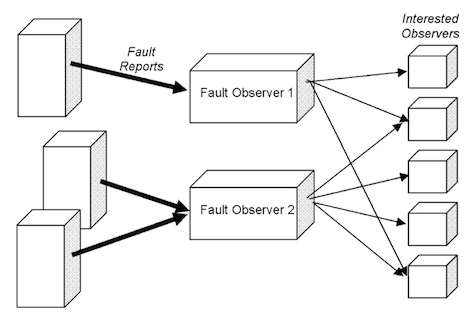
\includegraphics[width=\textwidth]{content/faulttolerance/images/U11_3_FaultObserver_2013.png}
	\caption{U11 3 FaultObserver 2013}
\end{figure}


Wichtig ist darauf zu achten das die Publisher einmalig oder als redundante Komponenten vorhanden sind und nicht mehrere Publisher die den selbe Information an einen Observer übermitteln. (führt zu Konfusion beim Observer und zu duplicated Code im System) Des Weiteren wäre es wünschenswert, dass bei einem Error der dazugehörige Fault mit geloggt wird um spätere Analysen zu vereinfachen.

\subsection{Schlussfolgerung}

Raportiere alle Errors an einen Fault Observer, welcher alle intressierten Parteien darüber informiert.
